\documentclass[tikz,border=2pt]{standalone}
\usepackage{tikz}
\usetikzlibrary{positioning}
\begin{document}
	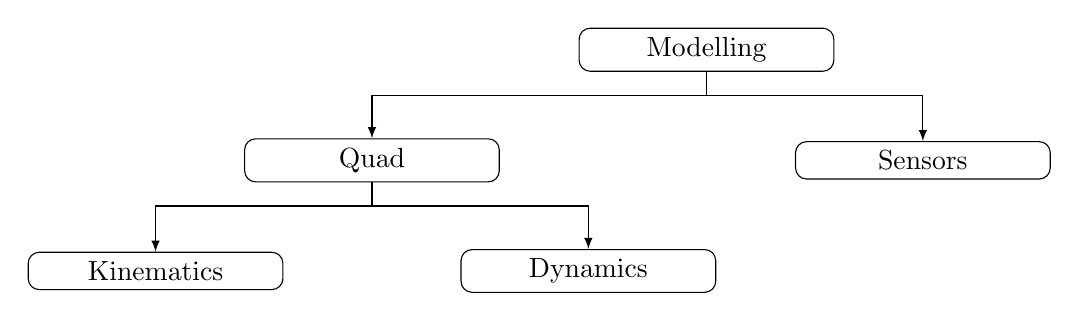
\begin{tikzpicture}[
	main/.style={rectangle, rounded corners, text centered, text width=3cm, draw=black},
	aux/.style={}
	]	
		\node (mod) [main] {Modelling};
			\node (aux4) [aux, below=of mod] {};	
			\node (quadmod) [main, left=2.5cm of aux4] {Quad};
				\node (aux7) [aux, below=of quadmod] {};
				\node (dynamics) [main, right=of aux7] {Dynamics};	
				\node (kinematics) [main, left=of aux7] {Kinematics};
			\node (sensorsmod) [main, right=of aux4] {Sensors};

	\draw [-latex] (mod.south)--++(0,-.3)-| (quadmod.north);
	\draw [-latex] (mod.south)--++(0,-.3)-| (sensorsmod.north);
	
	
	\draw [-latex] (quadmod.south)--++(0,-.3)-| (kinematics.north);
	\draw [-latex] (quadmod.south)--++(0,-.3)-| (dynamics.north);
	
	
	\end{tikzpicture}
\end{document}